\documentclass{article}

\usepackage{xcolor}
\usepackage{hyperref}
\definecolor{COLOR_MEAN}{HTML}{f0f0f0}
\definecolor{LINK_COLOR}{HTML}{636EFA}
\hypersetup{
	colorlinks=true,
	linkcolor=LINK_COLOR,
	urlcolor=LINK_COLOR,
	citecolor=LINK_COLOR,
}

% if you need to pass options to natbib, use, e.g.:
%     \PassOptionsToPackage{numbers, compress}{natbib}
% before loading neurips_2024


% ready for submission
%\usepackage{neurips_2024}


% to compile a preprint version, e.g., for submission to arXiv, add add the
% [preprint] option:
% \usepackage[preprint]{neurips_2024}


% to compile a camera-ready version, add the [final] option, e.g.:
\usepackage[final]{neurips_2024}


% to avoid loading the natbib package, add option nonatbib:
%    \usepackage[nonatbib]{neurips_2024}


\usepackage[utf8]{inputenc} % allow utf-8 input
\usepackage[T1]{fontenc}    % use 8-bit T1 fonts
\usepackage{hyperref}       % hyperlinks
% \usepackage{url}            % simple URL typesetting
\usepackage{xurl}
\usepackage{booktabs}       % professional-quality tables
\usepackage{amsfonts}       % blackboard math symbols
\usepackage{nicefrac}       % compact symbols for 1/2, etc.
\usepackage{microtype}      % microtypography
\usepackage[dvipsnames]{xcolor}
\usepackage{tabularx}
\usepackage{booktabs}
\usepackage{amsmath}
\usepackage{listings}
\usepackage{xspace}
\usepackage[capitalise]{cleveref}
\usepackage{multirow}
\usepackage{multicol}
\usepackage{subcaption}
\usepackage{graphicx}

\usepackage{algorithm}
\usepackage{algpseudocode}
\usepackage{mathrsfs}
\usepackage{tikz}

\usepackage[symbol]{footmisc}
\definecolor{ntured}{HTML}{D71440}
\hypersetup{
    colorlinks=true,     
    urlcolor=ntured,
}

\lstset{ 
  language=SQL,                     % the language of the code
  basicstyle=\ttfamily, % the size of the fonts that are used for the code
  numbers=left,                   % where to put the line-numbers
  numberstyle=\color{Blue},  % the style that is used for the line-numbers
  stepnumber=1,                   % the step between two line-numbers. If it is 1, each line
                                  % will be numbered
  numbersep=5pt,                  % how far the line-numbers are from the code
  backgroundcolor=\color{white},  % choose the background color. You must add \usepackage{color}
  showspaces=false,               % show spaces adding particular underscores
  showstringspaces=false,         % underline spaces within strings
  showtabs=false,                 % show tabs within strings adding particular underscores
  frame=single,                   % adds a frame around the code
  rulecolor=\color{black},        % if not set, the frame-color may be changed on line-breaks within not-black text (e.g. commens (green here))
  tabsize=2,                      % sets default tabsize to 2 spaces
  captionpos=b,                   % sets the caption-position to bottom
  breaklines=true,                % sets automatic line breaking
  breakatwhitespace=false,        % sets if automatic breaks should only happen at whitespace
  keywordstyle=\color{RoyalBlue},      % keyword style
  commentstyle=\color{YellowGreen},   % comment style
  stringstyle=\color{ForestGreen}      % string literal style
} 




\newcommand{\bplustree}{B+ tree\xspace}


% \title{SC3020 Project 1}


% The \author macro works with any number of authors. There are two commands
% used to separate the names and addresses of multiple authors: \And and \AND.
%
% Using \And between authors leaves it to LaTeX to determine where to break the
% lines. Using \AND forces a line break at that point. So, if LaTeX puts 3 of 4
% authors names on the first line, and the last on the second line, try using
% \AND instead of \And before the third author name.


% \author{
% }

\usepackage{graphicx}

\begin{document}
	
\begin{titlepage}
	\begin{figure}[!t]
		\centering
		
\includegraphics[width = 4.3in]{title/logo.pdf}
	\end{figure}
	
	\centering
	\huge{\textbf{SC3020 Database Systems Principles}}\\[0.2in]
	\huge{\textbf{Project 1 Report}}\\[2in]
        \small {Code: \url{https://bit.ly/SC3020Project1}} \\
        \small {Presentation Video: \url{https://bit.ly/SC3020Project1Video}}
	
	%	\LARGE{\textbf{YOUR NAME}}\\
	%	\normalsize{Matriculation number}\\[0.2in]
	
	\begin{table}[h]
		\centering
		\resizebox{\textwidth}{!}{%
			\begin{tabular}{lll}
				\toprule
				\textbf{Name} & \textbf{Email} & \textbf{Matric Number} \\
				\midrule
                    Cui Nan & C220133@e.ntu.edu.sg & U2221495L\\
				Pu Fanyi & FPU001@e.ntu.edu.sg & U2220175K \\
				Shan Yi & SH0005YI@e.ntu.edu.sg & U2222846C\\
                    Zhang Kaichen & ZHAN0564@e.ntu.edu.sg & U2123722J \\
                    Tian Yidong & YTIAN006@e.ntu.edu.sg & U2220492B \\
				\bottomrule
			\end{tabular}%
		}
	\end{table}

	
	
    
	
	%	\large{A Final Year Report submitted to Asian School of the Environment, Nanyang Technological University in partial fulfilment of the requirements for the Degree of }\\[0.1in]
	
	\vspace{0.5in}
    \LARGE{College of Computing and Data Science}\\
	\LARGE{Nanyang Technological University, Singapore}\\[0.3in]
	
	
	\LARGE{2024/2025 Semester 1}
	\newpage
\end{titlepage}
	
% \maketitle

% \begin{abstract}
%     lalala
% \end{abstract}


\section{Introduction}
\label{sec:intro}

This project focuses on the design and implementation of two key components of a database management system: storage and indexing.

Our report is structured as follows:

\begin{enumerate}
    \item First, we illustrate the design of our storage component, where data is stored in blocks on computer disks.
    \item Next, we describe the implementation of our \bplustree and the process of storing the index on the disk.
    \item Finally, we present the statistics and experimental results obtained using our database system.
\end{enumerate}


\section{Overview}
\label{sec:overv}

In this section, we will give a brief introduction on how our application functions.

\subsection{Pipeline Overview}

\begin{figure}
    \centering
    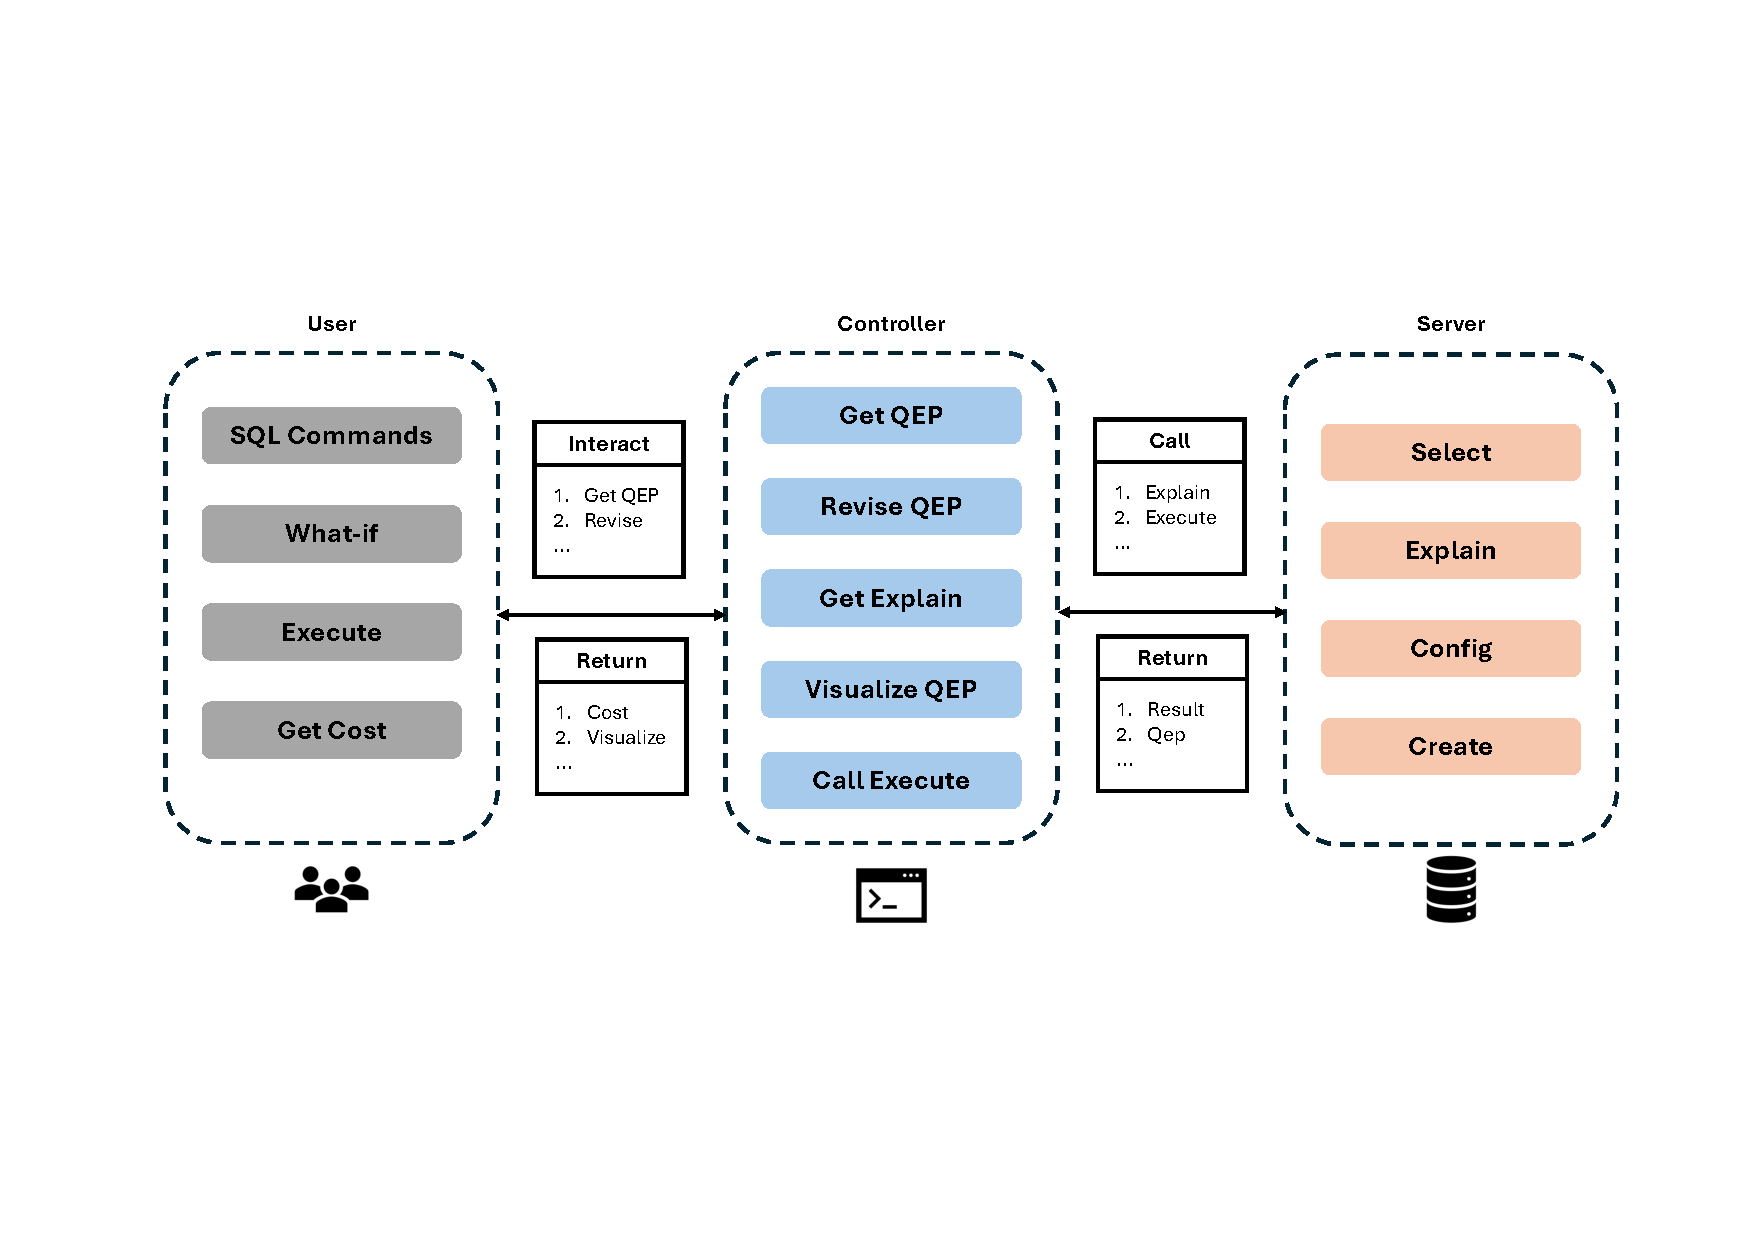
\includegraphics[width=1\linewidth]{figures/Pipeline.pdf}
    \caption{A overview of our pipeline. Where user can perform different operations and receive results from the controller and the server side. The user can freely decide when to execute the commands}
    \label{fig:pipeline}
\end{figure}

Our application mainly consist of three key components: \textbf{1)} A user-interface to allow user to interact with. \textbf{2)} A controller component that post the commands to the server and get the result. \textbf{3)} A database server that actually execute the commands and store the data.

Our application follows a modular pipeline that integrates a backend for query processing and a frontend for user interaction. The pipeline consists of several stages:

\paragraph{Database Connection} Users first connect to the PostgreSQL database through the GUI by providing connection details. If necessary, they can load a prepared dataset from the Internet and create the corresponding table in the database. This operation is performed only once and stores the \textit{tpch} dataset on the server.

\paragraph{Query Plan Retrieval} Users can input SQL queries or select examples through the GUI. Once a valid command is entered in the code panel, the QEP visualization is displayed. The execution and retrieval process algorithm is implemented efficiently, providing real-time details on costs, explanations, and tree visualizations. Further details about the algorithm are available in~\cref{sec:algo}.

\paragraph{Interactive What-If Analysis} Users can modify the query execution plan by changing join types or scan methods through the GUI. A list of options is provided, and changes are reflected in real time in the cost estimation and tree visualization. Planner settings are dynamically adjusted using SQL commands (e.g., \texttt{SET enable\_*}) based on the query planning configuration. Details of the algorithm are provided in~\cref{subsec:whatif-algo}.

\paragraph{Visualization and Explanation} After retrieving the QEP or the revised AQP from the server, the system parses it into a tree where each node represents an operation and its condition. This parsed tree is used to calculate the coordinates of the visualized QEP tree. We also provide natural language explanations derived from the tree using a post-order traversal. Each step is parsed according to a set of predefined rules and formats, then presented to the user.

\paragraph{Comparison and Results} Once the user is satisfied with their query plan, they can execute it to view the actual query results and query log. The system displays the query execution time, enabling users to validate performance.

\subsection{Application Structure}

The application is organized into the following key components:

\paragraph{Frontend} Gradio~\cite{abid2019gradio} is used as our frontend framework. The GUI accepts user inputs (connection details, SQL queries, and what-if modifications) and displays query plans, costs results and logs to the user. It also provides interactive dropdown menus for what-if analysis.

\paragraph{Backend} We adopted FastAPI~\cite{fastapi} as the framework to provide the backend server logic. The backend contacts the database in SQL commands, with Psycopg 3.

\paragraph{Database System} PostgreSQL~\citep{postgres_github} is selected as the Database system to manage our database. The database is established from TPC-H dataset~\cite{poess2000new}.\footnote{Version 3.0.1, retrieved from \href{https://www.tpc.org/TPC_Documents_Current_Versions/download_programs/tools-download-request5.asp?bm_type=TPC-H&bm_vers=3.0.1}{this link}, compiled with \texttt{Visual Studio 2022 version 17.10}.} To make it easier to reproduce our experiments on different devices, we have uploaded the data to Hugging Face Datasets~\cite{lhoest2021datasets}, which could be accessed by \href{https://huggingface.co/datasets/pufanyi/TPC-H}{this link}.

% \paragraph{Controllers of our system}
% \begin{enumerate}
%     \item  \textbf{Frontend (User Interface)}
%     \begin{itemize} 
%     \item Framework: Gradio~\cite{abid2019gradio} for GUI development.
%     \item Responsibilities: \begin{itemize} 
%     \item Accept user inputs (connection details, SQL queries, and what-if modifications).
%     \item Display query plans, costs, results, and logs.
%     \item Provide interactive dropdown menus for what-if analysis.
% \end{itemize}
%     \item Files: 
%     \begin{itemize}
%         \item \textit{interface.py}: Implements the Gradio GUI with components for database connection, query input, query plan visualization, and cost comparison. 
%         \item Other static files such as css, js, and html file for the base url
%     \end{itemize}  
% \end{itemize}


%     \item  \textbf{Backend (Query Processing)}
%     \begin{itemize} 
%     \item Framework: FastAPI~\citep{fastapi} for backend server logic.
%     \item Responsibilities: \begin{itemize} 
%     \item Establish database connections and manage \textit{TPC-H}~\cite{poess2000new} data.
%     \item Process user modifications to join and scan methods.
%     \item Pass SQL commands to PostgreSQL and retrieve results from PostgreSQL.
%     \item Provide APIs for the frontend to fetch query plans and costs.
% \end{itemize}
%     \item Files: \begin{itemize} 
%     \item \textit{project.py}: Main script for launching the server and handling CLI arguments.
%     \item \textit{whatif.py}: Contains algorithms for generating SQL commands based on user-selected join and scan methods.
%     \item \textit{tcph.py}: Contains the controller to interact with the database server.
%     \item \textit{ExecutionTree.py}: Contains all the code to parse the query plan into a tree.
%     \item \textit{visualizer.py}: Contains all the code to visualize the Execution Tree.
% \end{itemize}    

% \end{itemize}

%     \item  \textbf{Database}
%     \begin{itemize} 
%     \item System: PostgreSQL~\citep{postgres_github} with the \textit{TPCH} dataset.
%     \item Responsibilities: \begin{itemize} 
%     \item Execute SQL queries and provide query execution plans (QEPs).
%     \item Support advanced planner configurations for what-if analysis.
% \end{itemize}

% \end{itemize}

% \end{enumerate}

\subsection{Key Interaction Flow}

\paragraph{Database Connection} User connects to the database via GUI $\to$ FastAPI establishes the connection $\to$ PostgreSQL confirms the connection $\to$ Download the dataset from Hugging Face $\to$ Load data to the database.

\paragraph{Query Execution} User inputs query $\to$ Gradio sends request to FastAPI $\to$ FastAPI receives the query and send to PostgreSQL $\to$ PostgreSQL generates QEP and computes results and costs, then returns them to the FrontEnd.

\paragraph{What-If Analysis} User modifies join/scan types on the FrontEnd $\to$ Gradio sends modification request $\to$ FastAPI adjusts planner settings and send to PostgreSQL $\to$ PostgreSQL generates AQP and estimated costs.

\paragraph{Result Display} Results, costs, explains and logs are visualized in the GUI.


\section{Implementation Details}
\label{sec:algo}

\subsection{Parsing Query Plans and Tree Genreating}

A QEP is generated by PostgreSQL with the SQL statement:
\begin{lstlisting}
EXPLAIN <QUERY>;
\end{lstlisting}
A parser is created to parse the output of the generated QEP. We assume $\textsc{Parse}(p_i)$ function can extract the information of the plan and convert it to a node, $\textsc{Depth}(p_i)$ function can retrieve the depth of the plan. $\textsc{Depth}(p_0) = 0$.

The whole process generation QEP tree is DFS with backtracking, described in Algorithm \ref{alg:generate-execution-tree}.

The tree structure is explained in Section~\ref{sec:execution_tree_node} and \ref{sec:execution_tree}.

\begin{algorithm}[ht]
\caption{$\textsc{GenerateExecutionTree}(p)$}
\label{alg:generate-execution-tree}
\begin{algorithmic}[1]
\Require A list of strings representing query plans $p$ from PostgreSQL
\Ensure An \textsc{ExecutionTree} representing the QEP
\State $\mathcal{T}\leftarrow$ Empty Tree
\State $o\leftarrow \textsc{Parse}(p_0)$\Comment{$o$ is the current node}
\State $\textsc{Root}(\mathcal{T})\leftarrow o$\Comment{Set $o$ to be the root of $\mathcal{T}$}
\State $d\leftarrow 0$\Comment{Currently depth is $0$}
\For{$i\in 1\dots \textsc{Len}(p)-1$}\Comment{Enumerate remaining plans}
    \State $o'\leftarrow \textsc{Parse}(p_i)$\Comment{Current node}
    \State $d'\leftarrow \textsc{Depth}(p_i)$\Comment{Current depth}
    \While{$d'\le d$}\Comment{Backtrack to Find Parent of $o$}
    \State $o\leftarrow\textsc{Parent}(o)$
    \State $d\leftarrow d - 1$
    \EndWhile
    \State $\textsc{Parent}(o')\leftarrow o$\Comment{Set the parent of $o'$ to $o$}
    % 就是我感觉我们这个 algo 是不是应该强调建树的过程,而不是 parse 的过程
    % \If{`\texttt{:}'$\in \ell$}\Comment{$\ell$ contains a condition}
    %     \State Add the condition to the current node
    % \ElsIf{`\texttt{->}'$\in\ell$}\Comment{$\ell$ contains an operation}
    %     \State Create a new node for the operation
    %     \State Determine the node's level in the tree based on indentation (arrow positions)
    %     \State Link the node to its parent in the tree hierarchy
    % \EndIf
\EndFor

\State \Return $\mathcal{T}$
\end{algorithmic}
\end{algorithm}


\subsection{\textsc{ExecutionTreeNode} Class}
\label{sec:execution_tree_node}

The \textsc{ExecutionTreeNode} class represents a single node in the execution tree. Each node corresponds to a query operation (e.g., Hash Join, Seq Scan) and includes metadata like costs and conditions associated with that query operation.

Table \ref{tab:ExecutionTreeNode_attributes} lists the key attributes and methods for \textsc{ExecutionTreeNode}.

\begin{table}[ht]
    \centering
    \begin{tabular}{l|l}
    \toprule
        \textbf{Attributes / Methods} & \textbf{Description} \\
    \midrule
        Operation & The query operation. \\
        Conditions & Filters or keys associated with the operation.\\
        Startup Cost & Startup cost for the operation.\\
        Total Cost & Total cost for the operation.\\
        Children & Child nodes representing sub-operations.\\
    \midrule
        Set Operation & Parses the operation and perform estimation.\\
        Natural Language & Converts the operations into a human-readable format.\\
        Explain & Returns the detailed estimation to the operation. \\
    \bottomrule
    \end{tabular}
    \caption{Key Attributes and Methods for \textsc{ExecutionTreeNode}}
    \label{tab:ExecutionTreeNode_attributes}
\end{table}


\subsection{\textsc{ExecutionTree} Class}
\label{sec:execution_tree}

The \textsc{ExecutionTree} class organizes query operations into a hierarchical structure, allowing traversal and cost analysis. Table \ref{tab:ExecutionTree_attributes} lists key attributes and methods of \textsc{ExecutionTree}.

\begin{table}[ht]
    \centering
    \begin{tabular}{l|l}
    \toprule
        \textbf{Attributes / Methods} & \textbf{Description} \\
    \midrule
        Root & The root node of the tree. \\
    \midrule
        Traversal & Return nodes based on the order of operations.\\
        Get Cost & Aggregates the startup and total costs of all nodes.\\
    \bottomrule
    \end{tabular}
    \caption{Key Attributes and Methods for \textsc{ExecutionTree}}
    \label{tab:ExecutionTree_attributes}
\end{table}

The \textsc{Traversal} method uses post-order traversal methods to return nodes. $\textsc{Traversal}(o, \ell)$ means the current node is $o$, and the answer list is $\ell$. shown in Algorithm~\ref{algo:traversal}. The total cost and startup cost inside a tree is calculated by summing all the total cost and startup cost for each node in it.

\subsection{Interactive What-If Analysis}
\label{subsec:whatif-algo}

We explored generating alternative query plans by applying user-defined modifications to join and scan methods. \textsc{PrepareJoinCommand} and \textsc{PrepareScanCommand} generate \texttt{SET} commands to control PostgreSQL planner configurations. For instance, when a user selects \texttt{HASH\_JOIN}:
\begin{lstlisting}
SET enable_hashjoin = ON;
SET enable_mergejoin = OFF;
SET enable_nestloop = OFF;
\end{lstlisting}

\begin{algorithm}
	\caption{$\textsc{Traversal}(o, \ell)$}
    \label{algo:traversal}
	\begin{algorithmic}
        \For{$s\in\textsc{Son}(o)$}
            \State $\textsc{Traversal}(s, \ell)$
        \EndFor
        \State$\textsc{Append}(\ell, o)$
	\end{algorithmic} 
\end{algorithm}

This ensures that PostgreSQL uses only the specified join type when generating the QEP. Similarly, we can disables other scan methods and enables only index-based scanning by producing:

\begin{lstlisting}
SET enable_bitmapscan = OFF;
SET enable_indexscan = OFF;
SET enable_indexonlyscan = ON;
SET enable_seqscan = OFF;
\end{lstlisting}

\subsection{QEP Visualizer}

QEP Visualizer converts a \textsc{ExecutionTree} to a plot. Firstly,  We consider the tree as a planar graph and calculate the coordinates of each node using igraph~\cite{igraph}. The specific calculation method is mentioned in \cite{reingold1981tidier}. Then, Based on these coordinates, we perform scaling transformations to adapt them to the screen. Using Plotly~\cite{plotly}, we plot the nodes and edges in a Cartesian coordinate system. Finally, we remove the coordinate axes to generate an image of the tree.

To display information for each node concisely, we use symbols to represent each node, with the specific mappings listed in Table~\ref{tab:operation_description}. Detailed information about that node is displayed when the mouse hovers over a specific node.

\begin{table}[ht]
    \centering
    \begin{tabular}{c|c|l}
    \toprule
        \textbf{Operation} & \textbf{Symbol} & \textbf{Description} \\
    \midrule
        Aggregate & $\gamma$ & Performs aggregation operations like \texttt{SUM}, \texttt{AVG}, etc. \\
        Hash Join & $\Join_H$ & Joins two tables using a hash-based method. \\
        Merge Join & $\Join_M$ & Joins two sorted tables using a merge-based approach. \\
        Seq Scan & $\sigma$ & Sequentially scans all rows in a table. \\
        Index Scan & $\sigma_I$ & Scans rows using an index for faster lookup. \\
        Bitmap Heap Scan & $\sigma_B$ & Uses a bitmap index for efficient range scans. \\
        Sort & $\tau$ & Sorts the rows based on specified columns. \\
        Hash & $H$ & Creates a hash table for efficient data access. \\
        Gather Merge & $\gamma_M$ & Merges results from multiple parallel workers. \\
        Materialize & $M$ & Stores intermediate results in memory for reuse. \\
        Append & $\cup$ & Combines rows from multiple sources into one output. \\
        Unique & $\delta$ & Removes duplicate rows. \\
        Group & $\gamma$ & Groups rows by specific column(s) for aggregation. \\
        Window & $\omega$ & Computes window functions like \texttt{RANK}, \texttt{ROW\_NUMBER}, etc. \\
        Limit & $L$ & Restricts the output to a specified number of rows. \\
        Unknown Operation & $o$ & Represents an operation that is not recognized. \\
    \bottomrule
    \end{tabular}
    \caption{Operations and their corresponding symbols.}
    \label{tab:operation_description}
\end{table}


% \textbf{Flexibility for Various What-If Scenarios:}
% The code uses registries (\texttt{JOIN\_REGISTRY} and \texttt{SCAN\_REGISTRY}) to define supported join and scan types, making it easy to extend or customize. Users can combine different strategies for testing without modifying the core logic.

% \textbf{Core Steps in What-If Analysis:}
% \begin{enumerate}
%     \item \textbf{User Modifies the QEP}: Users interactively specify the desired join or scan type changes. The code translates these inputs into PostgreSQL configuration commands.
%     \item \textbf{Generate a New QEP}: The generated commands are executed, guiding PostgreSQL to produce a new Alternative Query Plan (AQP) reflecting the user’s modifications.
%     \item \textbf{Compare QEP and AQP}: By comparing the costs of the original QEP and the modified AQP, users can evaluate the impact of their changes on query performance.
% \end{enumerate}




\section{Case Study}
\label{sec:application}

In this section, we present case studies demonstrating the use of our project. One complex example is highlighted to showcase the correctness and effectiveness of our application. We present more examples that can also be executed directly using our application. In application, you can also hover the mouse on each node for more infomation.

\newpage

\begin{lstlisting}
SELECT
    n_name,
    SUM(l_extendedprice * (1 - l_discount)) AS revenue
FROM
    customer,
    orders,
    lineitem,
    supplier,
    nation,
    region
WHERE
    c_custkey = o_custkey
    AND l_orderkey = o_orderkey
    AND l_suppkey = s_suppkey
    AND c_nationkey = s_nationkey
    AND s_nationkey = n_nationkey
    AND n_regionkey = r_regionkey
    AND r_name = 'ASIA'
    AND o_orderdate >= '1994-01-01'
    AND o_orderdate < '1995-01-01'
    AND c_acctbal > 10
    AND s_acctbal > 20
GROUP BY
    n_name
ORDER BY
    revenue DESC;
\end{lstlisting}

\begin{figure}[ht]
    \centering
    \begin{subfigure}[b]{0.49\linewidth}
        \centering
        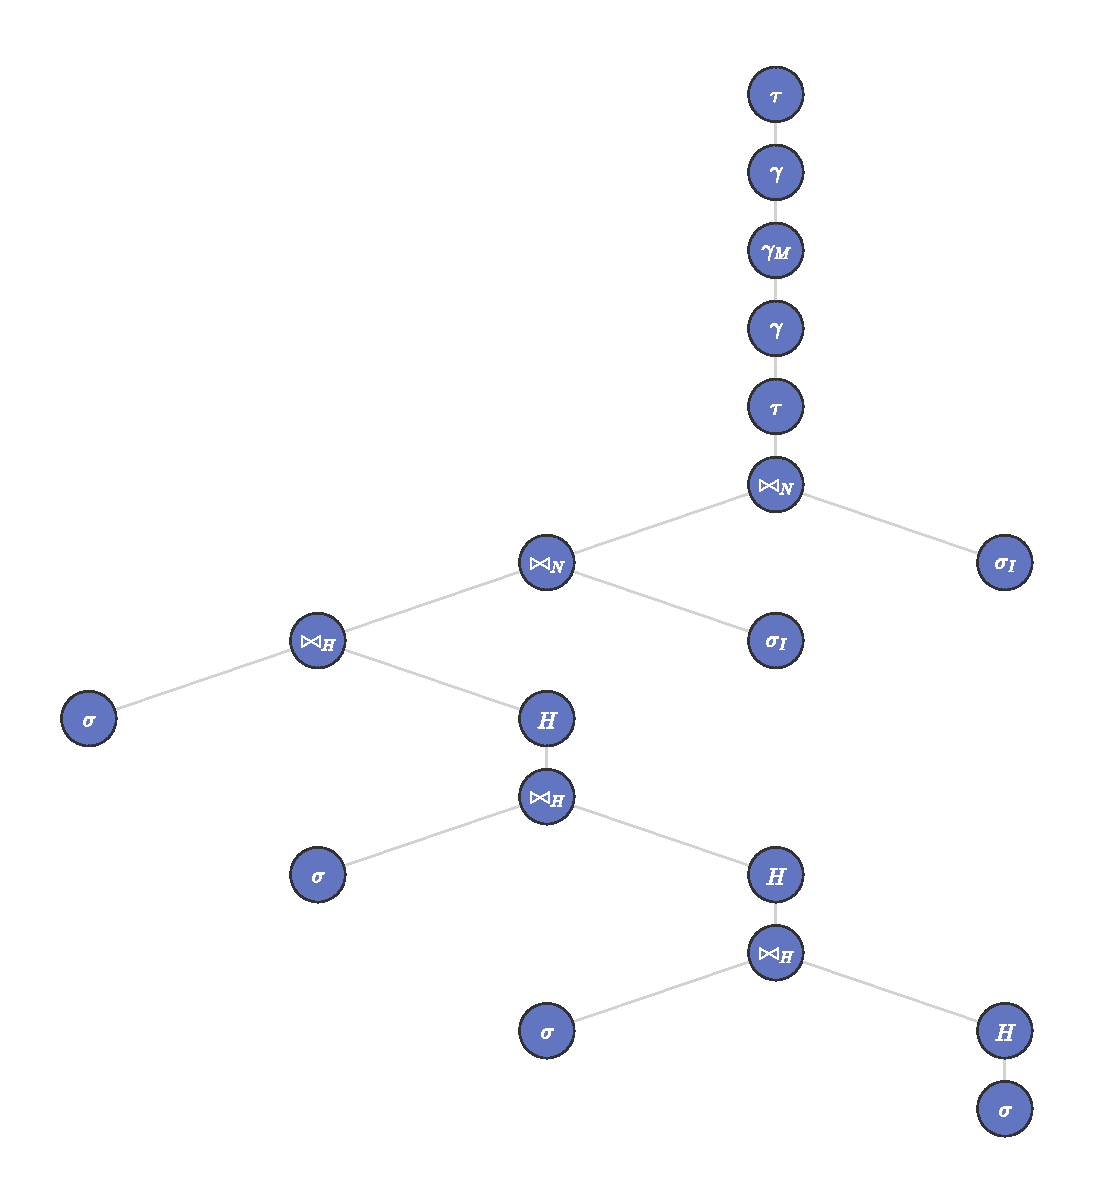
\includegraphics[width=\linewidth]{figures/example1_query_plan.pdf}
        \caption{The visualization of the example query plan using the default settings. The database can freely choose to use which scan type or join type.}
        \label{fig:vis-example-default}
    \end{subfigure}
    \hfill
    \begin{subfigure}[b]{0.49\linewidth}
        \centering
        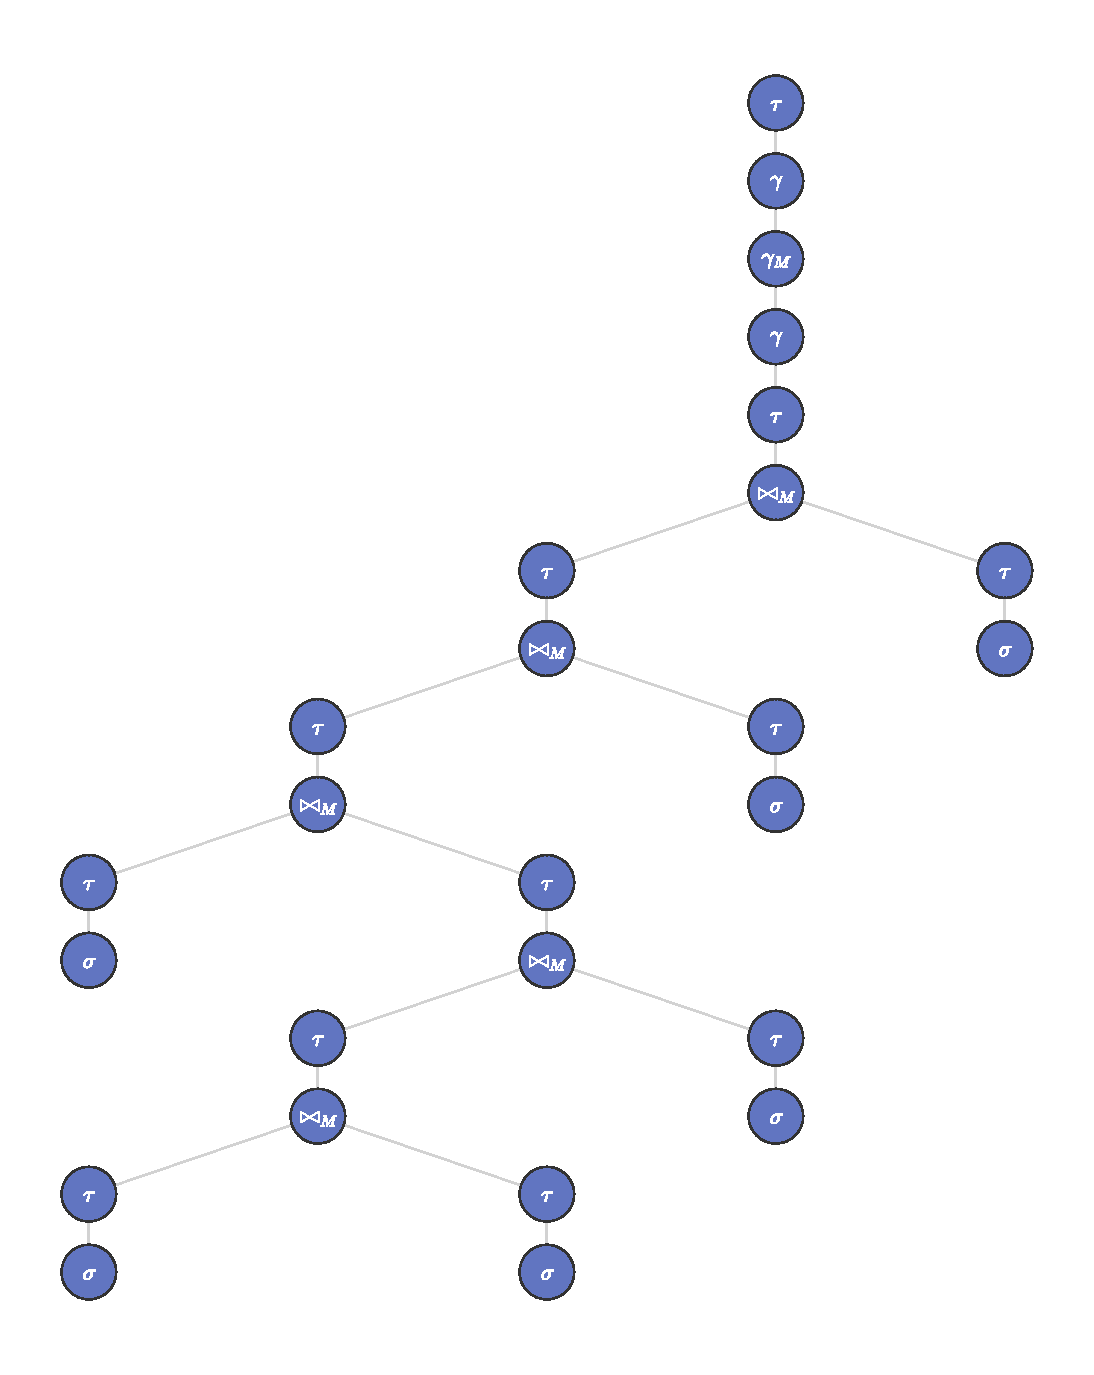
\includegraphics[width=\linewidth]{figures/example1_query_plan_seq_mj.pdf}
        \caption{The visualization of the example query plan by setting the scan method to Sequential Scan and join method to Merge Join.}
        \label{fig:vis-example-ss-mj}
    \end{subfigure}
    \caption{Comparison of the example query plan visualizations.}
    \label{fig:vis-example-comparison}
\end{figure}

\begin{table}[h]
\centering
\begin{tabular}{lll}
\toprule
         & Startup Cost & Total Cost \\
\midrule
Original & 815194.52    & 1434838.82 \\
Revised  & 6592161.29   & 6813958.6 \\
\bottomrule
\end{tabular}
\label{tab:cost-comp}
\caption{The estimated cost for different QEP}
\end{table}

\paragraph{QEP and AQP comparisons} The original Query Execution Plan (QEP) for the above case study example uses scanning method of Index Scan and Sequential Scan to perform selecting; it also performs join using Nested Loop Join and Hash Join; the QEP is shown in~\cref{fig:vis-example-default}. Then the user tests the changes that can be caused by modifying scan method to Sequential Scan and join method to Nested Loop Join, which generates an AQP; the AQP is shown in~\cref{fig:vis-example-ss-mj}. As observed from the above graphs for query plans, the AQP is different from the initial QEP in tree structure and operator sequences. The revised QEP is forced to use sequential scan and merge join for each of the node. We show their estimation cost in~\cref{tab:cost-comp}.



\section{Conclusion and Limitation}
\label{sec:conclusion and limitation}

Our software effectively utilizes an interface to allow users to interactively invoke the PostgreSQL database system for query execution and cost evaluation, as well as to visualize the effect of changing the join or the scanning methods on query execution plan and cost of plans. 

By leveraging structured tree representations and intuitive visualizations of plan in tree structure view, it helps the users to understand the complex task of query generation and optimization. Make the understanding process less difficult through visual demonstration of query execution process.

\paragraph{Limitations} Our application leverages PostgreSQL's configuration options for query plans to enforce the use of specific scan or join methods when generating the QEP. However, this approach cannot precisely modify individual nodes within the QEP, as it uniformly applies the specified method to all join or scan nodes. To fine-tune the processing logic for each node, extensions such as \textit{pg\_hint\_plan} can be utilized.

\section{Use of AI tools}
We used ChatGPT to help us refine the paragraph, and picked the grammar mistakes in the report. All the report draft and graphs were written and designed by us.

Part of the hardcode logics, such as if-else statement for the node symbol, which require repeated work are being done by the code pilot. We coded all of our core components by ourselves.


\newpage

\bibliographystyle{plain} % or another style like apalike, abbrvnat, etc.
\bibliography{references/ref} % assumes you have a references.bib file

% \newpage
% \appendix
% \input{sections/appendix}


\end{document}